% a mashup of hipstercv, friggeri and twenty cv
% https://www.latextemplates.com/template/twenty-seconds-resumecv
% https://www.latextemplates.com/template/friggeri-resume-cv

% !TeX program = xelatex 

\documentclass[lighthipster]{simplehipstercv}
% available options are: darkhipster, lighthipster, pastel, allblack, grey, verylight, withoutsidebar
% withoutsidebar
\usepackage[utf8]{inputenc}
\usepackage[default]{raleway}
\usepackage[margin=1cm, a4paper]{geometry}
\usepackage{hyperref}
\usepackage{textcomp} 

% other packages
\usepackage{subfigure}
\usepackage{latexsym,amsmath,xcolor,multicol,booktabs,calligra}
\usepackage{graphicx,pstricks,listings,stackengine}
\usepackage{quoting}
\usepackage{tcolorbox}

% 支持中文的设置
\usepackage{xeCJK}
\usepackage{fontspec}
\setCJKmainfont[ItalicFont=思源宋体,BoldFont=SourceHanSerifSC-Bold]{Source Han Serif SC}
\newcommand{\KaiTi}{\CJKfontspec{楷体}}%用命令\fzkaiti调用方正楷体简体

%------------------------------------------------------------------ Variablen

\newlength{\rightcolwidth}
\newlength{\leftcolwidth}
\setlength{\leftcolwidth}{0.23\textwidth}
\setlength{\rightcolwidth}{0.75\textwidth}

% 定义自定义命令来创建隐藏网址的超链接
\newcommand{\hiddenlink}[2]{%
	\href{#1}{\texttt{#2}}%
}

%------------------------------------------------------------------
\title{New Simple CV}
\author{\LaTeX{} Ninja}
\date{June 2019}

\pagestyle{empty}
\begin{document}
	
	
	\thispagestyle{empty}
	%-------------------------------------------------------------
	
	\section*{Start}
	
	\simpleheader{headercolour}{王}{升平}{软件部副经理}{white}
	
	
	
	%------------------------------------------------
	
	% this has to be here so the paracols starts..
	\subsection*{}
	\vspace{4em}
	
	\setlength{\columnsep}{1.5cm}
	\columnratio{0.18}[0.8]
	\begin{paracol}{2}
		\hbadness5000
		%\backgroundcolor{c[1]}[rgb]{1,1,0.8} % cream yellow for column-1 %\backgroundcolor{g}[rgb]{0.8,1,1} % \backgroundcolor{l}[rgb]{0,0,0.7} % dark blue for left margin
		
		% \paracolbackgroundoptions
		
		% 0.9,0.9,0.9 -- 0.8,0.8,0.8
		
		
		\footnotesize
		{\setasidefontcolour
			\flushright
			\begin{center}
				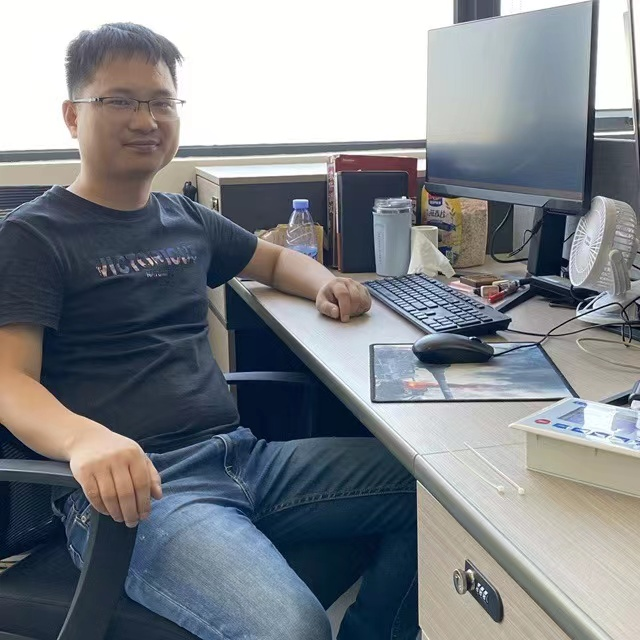
\includegraphics[width=\linewidth]{ShowMe.jpg}
			\end{center}
			\bigskip
			
			\bg{cvgreen}{white}{关于我}\\[0.5em]
			
			{
				\footnotesize
				10+年C++开发经验\\
				\tiny
				(3+年MFC,9+年Qt)\\
				\footnotesize
				3+年10人团队管理经验\\
				\tiny
				(开发/算法/测试 -- 敏捷开发)
			}
			\bigskip
			
			\bg{cvgreen}{white}{个人信息} \\[0.5em]
			王升平\\
			籍贯: 湖北\\ 
			1989
			
			\bigskip
			
			\bg{cvgreen}{white}{专业领域} \\[0.5em]
			
			~•~ 高性能交互界面开发\\ ~•~ 内存性能调优\\ ~•~ 跨平台移植\\ ~•~ 程序构架设计
			
			\bigskip
			
			
			
			\bigskip
			
			\bg{cvgreen}{white}{专业兴趣}\\[0.5em]
			C++逆向代码还原\\
			WinDbg Dump分析\\
			技术分享
			\bigskip
			
			\bg{cvgreen}{white}{技术追求方向}\\[0.5em]
			
			{
				\footnotesize
				项目构架管理\\
				\tiny
				(自上向下跟进前沿技术框架)\\
				\footnotesize
				逆向工程\\
				\tiny
				(自下向上深耕计算机原理)
			}
			\bigskip
			
			\vspace{4em}
			
			\infobubble{\faGithub}{cvgreen}{white}{thinct}
			
			\phantom{turn the page}
			
			\phantom{turn the page}
		}
		%-----------------------------------------------------------
		\switchcolumn
		
		\small
		\section*{公司简历}
		
		\begin{tabular}{r| p{0.5\textwidth} c}
			\cvevent{2021--至今}{\hiddenlink{https://www.thunderlaser.cn/}{东莞市雷宇激光设备有限公司}}{GuangDong}{DongGuan \color{cvred}}{\begin{enumerate}
					\item 组建软件部团队
					\item 将LaserMaker由MFC移植Qt,实现跨平台和新特性研发.
			\end{enumerate}} {logo_TL.png} \\
			\cvevent{2012--2021}{\hiddenlink{https://www.optmv.com/}{广东省奥普特股份有限公司(股票号:688686)}}{GuangDong}{DongGuan \color{cvred}}{\begin{enumerate}
					\item 负责维护视觉项目
					\item 专注研发SciSmartCamera 2.0/3.0软件
			\end{enumerate}} {logo_OPT.png} 
		\end{tabular}
		
		\vspace{1em}
		
		\section*{产品简介}
		\begin{tabular}{r| p{0.5\textwidth} c}
			\cvevent{2022--至今}{\hiddenlink{https://www.lasermaker.com.cn/}{Laser Maker V2.0}}{GuangDong}{DongGuan \color{cvred}}{\scriptsize \linespread{1.5} \selectfont LaserMaker是一款为创客科教市场研发的激光绘图建模软件。不仅仅是一款易用的绘图软件,还将激光工艺与模拟造物融为一体。LaserMaker便于快速建模,
				还能让使用者加深对激光工艺和加工原理的认识。作为一款教学性强的建模软件,同时适用于理论与实操学习。}{lasermaker.png} \\
			\vspace{1.0em}
			\cvevent{2012--2021}{\hiddenlink{http://net.bangong.cn:8771/content/details67_628.html}{SciSmart V2.0\&V3.0}}{GuangDong}{DongGuan \color{cvred}}{\scriptsize \linespread{1.5} \selectfont SciSmart智能视觉软件三代(以下简称SciSmart3)是一款简单易用、功能齐全、性能稳定的智能型视觉系统软件。SciSmart3由OPT自主研发,集成了预处理、定位、测量、检测、识别、3D聚焦、自动对焦、3D结构光测量、双目立体测量、光度立体技术等一系列图像处理工具。兼容市面上可见的主流相机品牌和GeniCam协议。支持串口、TCP等多种通讯模式及主流的通讯协议,能够方便的与各品牌运动控制设备建立数据交互。
				
				SciSmart3采用图形化编程代替代码编程,从而缩短项目开发周期。流程设计、流程复用方式以及流程与事件触发机制的组合方式,能够简化视觉检测项目流程。}{logo_OPT.png} \\
		\end{tabular}
		\vspace{1em}
	
		\begin{minipage}[t]{0.3\textwidth}
			\section*{编程语言}
			\begin{tabular}{r @{\hspace{0.5em}}l}
				\bg{headerfontboxfont}{iconcolour}{VC++} &  \barrule{0.4}{0.5em}{cvpurple}\\
				\bg{headerfontboxfont}{iconcolour}{C++} & \barrule{0.55}{0.5em}{cvgreen} \\
				\bg{headerfontboxfont}{iconcolour}{Qt} & \barrule{0.5}{0.5em}{cvpurple} \\
				\bg{headerfontboxfont}{iconcolour}{Python} & \barrule{0.1}{0.5em}{cvpurple} \\
				\bg{headerfontboxfont}{iconcolour}{ASM} & \barrule{0.1}{0.5em}{cvpurple} \\
			\end{tabular}
		\end{minipage}	\hfill
		\begin{minipage}[t]{0.3\textwidth}
		\section*{调试工具}
		\begin{tabular}{r @{\hspace{0.5em}}l}
			\bg{headerfontboxfont}{iconcolour}{VisualStudio} & \barrule{0.55}{0.5em}{cvgreen} \\
			\bg{headerfontboxfont}{iconcolour}{WinDbg} &  \barrule{0.3}{0.5em}{cvpurple}\\
			\bg{headerfontboxfont}{iconcolour}{X64Dbg} & \barrule{0.25}{0.5em}{cvpurple} \\
			\bg{headerfontboxfont}{iconcolour}{IDA Pro} & \barrule{0.25}{0.5em}{cvpurple} \\
		\end{tabular}
		\end{minipage}
		
		\vspace{1em}
		
		
		\begin{minipage}[t]{0.7\textwidth}
			\section*{个人领导团队经历}
			
			\begin{minipage}[t]{\textwidth}
				\begin{minipage}[t]{0.25\textwidth}
					\textbf{\underline{制定项目研发流程}}
					\begin{enumerate}
						\item 分析需求
						\item 制定开发计划
						\item 评估项目周期
						\item 任务分解和派发
						\item 组织测试
						\item 验收
					\end{enumerate}
				\end{minipage} 
				\hfill
				\begin{minipage}[t]{0.33\textwidth}
					\textbf{\underline{敏捷开发管理}}
					\begin{enumerate}
						\item 使用禅道做敏捷开发管理
						\item 项目集创建和管理
						\item 产品需求分析管理
						\item 组建测试团队并进行BUG测试管理
						\item 进度和风险管理
					\end{enumerate}
				\end{minipage} 
				\hfill
				\begin{minipage}[t]{0.35\textwidth}
					\textbf{\underline{人才招聘和培养}}
					\begin{enumerate}
						\item 招聘人才
						\item Qt零基础培养,3\textasciitilde6个月后可独挡一面
						\item 项目难点分析经验分享
						\item 协助同事攻坚,并分享思路
					\end{enumerate}
				\end{minipage}
				\bigskip
			\end{minipage}
		\end{minipage}
		
		
		\vspace{1em}
		
		\vfill{} % Whitespace before final footer
		
		%----------------------------------------------------------------------------------------
		%	FINAL FOOTER
		%----------------------------------------------------------------------------------------
		\setlength{\parindent}{0pt}
		\begin{minipage}[t]{\rightcolwidth}
			\begin{center}\fontfamily{\sfdefault}\selectfont \color{black!70}
				{\icon{\faMapMarker}{cvgreen}{} GuangDong/DongGuan \icon{\faPhone}{cvgreen}{} 13265599720 \icon{\faAt}{cvgreen}{} \protect\url{thinct_123@foxmail.com}
				}
			\end{center}
		\end{minipage}
		
	\end{paracol}
	
	\clearpage
	
	\begin{minipage}[t]{\textwidth}
		\section*{开发经验:SciSmart负责的主要模块}
		\begin{minipage}[t]{0.5\textwidth}
			\begin{flushleft}
				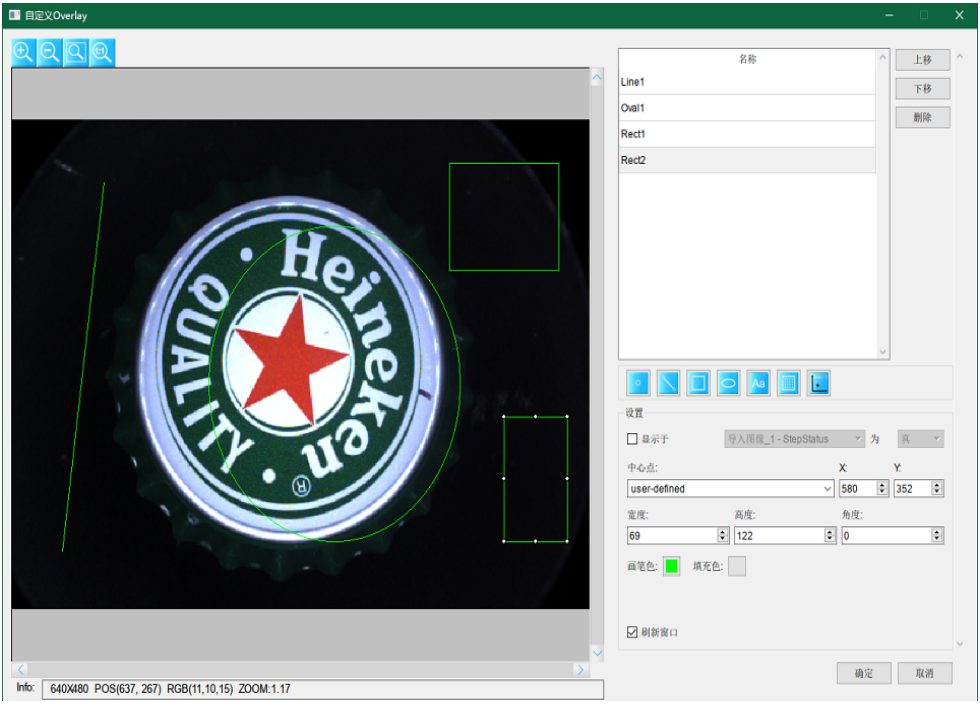
\includegraphics[width=0.8\linewidth]{PrjOPT_1.png}
				\begin{enumerate}
					\item 显示效率高
					\item 缩放之后图元线条线宽不变
					\item 支持Region效果
				\end{enumerate}
				本控件是SciCamera软件的最重要的界面之一。主要是支持显示图片和各种功能矢量图图元。软件所有的图像操作交互都是在该界面上完成的。作为一个UI控件,线程安全性高,并且显示图片的速度快。
			\end{flushleft}
		\end{minipage}
		\hspace*{1.6em}
		\begin{minipage}[t]{0.5\textwidth}
			\begin{flushleft}
				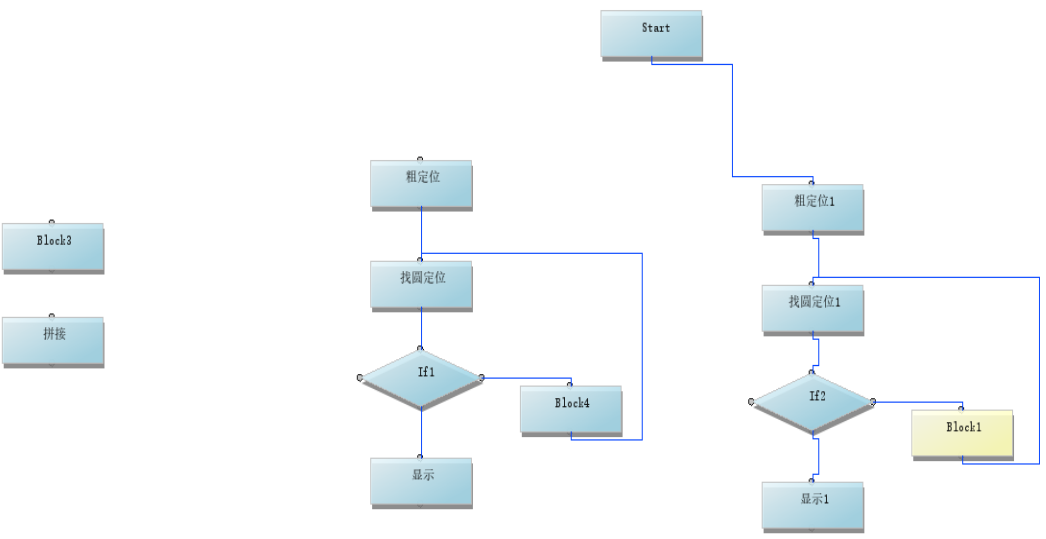
\includegraphics[width=0.8\linewidth]{PrjOPT_2.png}
				\begin{enumerate}
					\item 线程判断功能。能有效规避现场人员错误使用\\线程的问题
					\item 逻辑判断完整且灵活
				\end{enumerate}
				\vspace{0.8em}
				本控件是SciCamera软件的最重要的界面之一。主要是完成所有模块的流程逻辑任务,快速实现客户非标任务。流程算子块可以完成顺序,分支控制等基本功能。对线程有稳定性支持,可以有效提升任务执行效率,且能让新手有效避免线程安全这类复杂性问题。
			\end{flushleft}
		\end{minipage}
		
		\vfill
		\vspace{2em}
		
		\begin{minipage}[t]{0.5\textwidth}
		\begin{flushleft}
			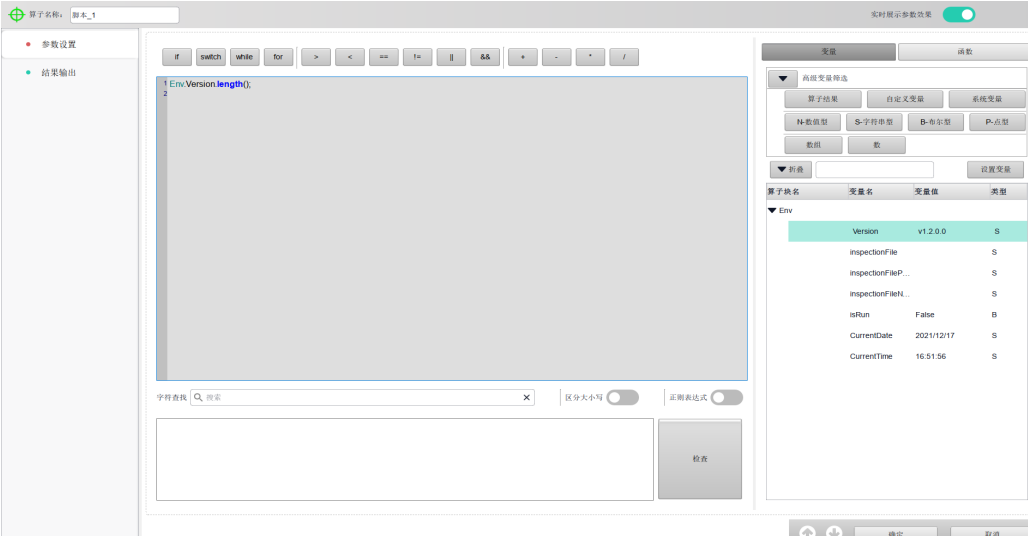
\includegraphics[width=0.8\linewidth]{PrjOPT_3.png} 
			\vfill
			\vspace{5em}
			C++和脚本混编,提高公共平台软件的灵活性。在非标项目中,可以灵活修改通信格式进行与不同PLC格式通讯协议。
			\\本控件是SciCamera软件的最重要的模块之一。主要是解决各个模块数据的简单逻辑处理,使不同模块在流程图的逻辑部署下,数据能有效的按需求传递。
		\end{flushleft}
		\end{minipage}
		\hspace*{1.6em}
		\begin{minipage}[t]{0.5\textwidth}
		\begin{flushleft}
			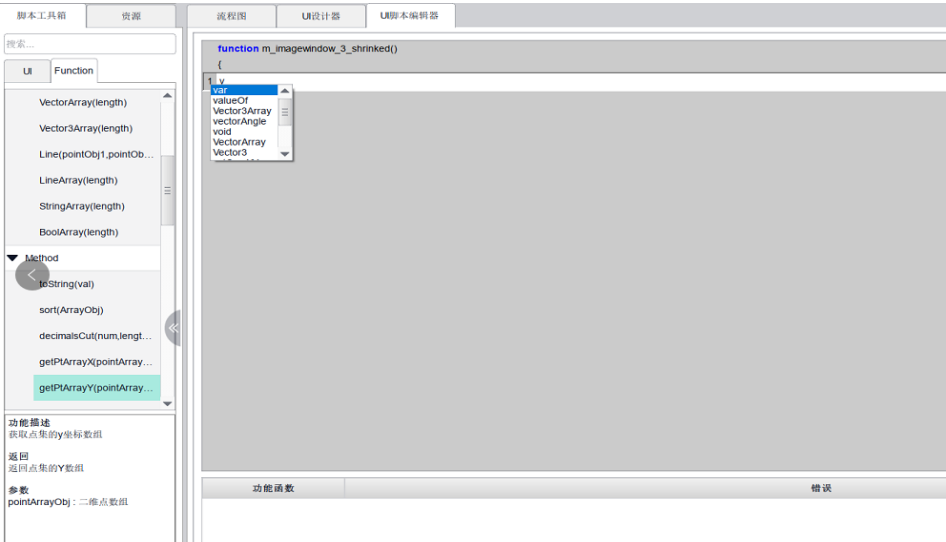
\includegraphics[width=0.8\linewidth]{PrjOPT_4.png}
			\begin{enumerate}
				\item IDE编辑控件开发
				\item Qt与脚本信号绑定
			\end{enumerate}
			本控件是SciCamera软件的最重要的模块之一。主要是目标使完成非标软件的界面快速定制化。本软件中有类似ot Creator设计师一样的界面拖拽定制界面的功能模块,而这个UI脚本就是作为该界面下响应事件的代码模块。本模块有脚本交互能力,有报错信息,其编码界面有对象补全和候选对象补全等能力。
		\end{flushleft}
		\end{minipage}
		\bigskip
	\end{minipage}
	\vspace{1em}
	
	\begin{minipage}[t]{\textwidth}
		\section*{开发经验:LaserMaker主要负责人}
		\begin{minipage}[thbp]{0.3\textwidth}
			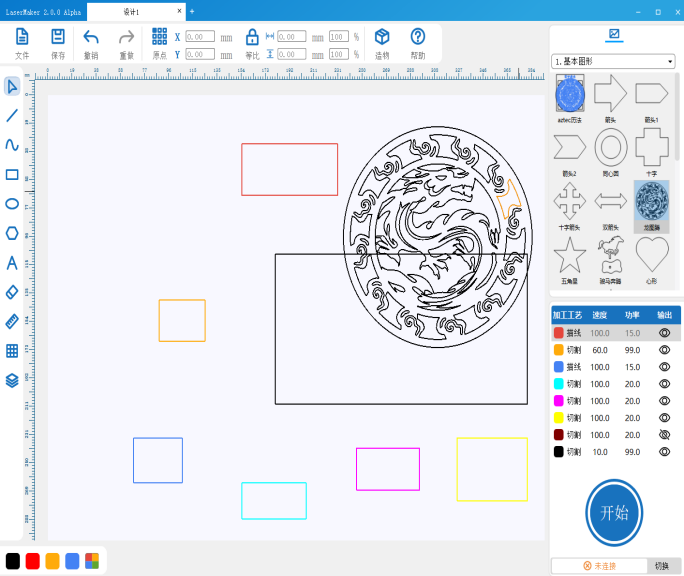
\includegraphics[width=\linewidth]{PrjTL_1.png}
		\end{minipage} \hfill
		\begin{minipage}[thbp!]{0.6\textwidth}
			\begin{enumerate}
				\item 带领团队完成从MFC到Qt的移植工作
				\item 主要解决大图像或者复杂矢量图显示等性能优化问题
				\item 解决程序崩溃问题
			\end{enumerate}
			LaserMaker是一款为创客科教市场研发的激光绘图建模软件。不仅仅是一款易用的绘图软件,还将激光工艺与模拟造物融为一体。LaserMaker便于快速建模,
			还能让使用者加深对激光工艺和加工原理的认识。作为一款教学性强的建模软件,同时适用于理论与实操学习。
		\end{minipage}
		\bigskip
	\end{minipage}
	
	\vspace{0.1em}
	
	\vfill{} % Whitespace before final footer
	
	%----------------------------------------------------------------------------------------
	%	FINAL FOOTER
	%----------------------------------------------------------------------------------------
	\setlength{\parindent}{0pt}
	\begin{minipage}[t]{\linewidth}
		\begin{flushright}\fontfamily{\sfdefault}\selectfont \color{black!70}
			{\icon{\faMapMarker}{cvgreen}{} GuangDong/DongGuan \icon{\faPhone}{cvgreen}{} 13265599720 \icon{\faAt}{cvgreen}{} \protect\url{thinct_123@foxmail.com}
			}
		\end{flushright}
	\end{minipage}
	
	\begin{minipage}[t]{\textwidth}
		\section*{开发经验:视觉软件开发}
		
		\begin{minipage}[t]{\textwidth}
			\begin{minipage}[thbp]{0.3\textwidth}
				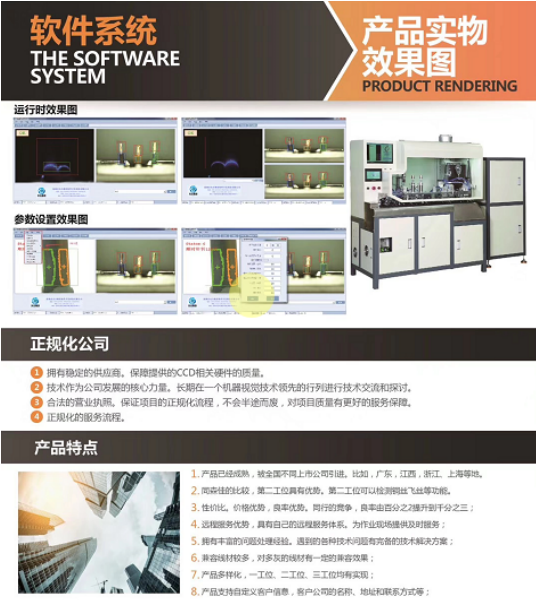
\includegraphics[width=\linewidth]{PrjMy_1.png}
			\end{minipage} 
			\hfill
			\begin{minipage}[thbp]{0.6\textwidth}
				\textbf{\underline{线材分线系统}}
				\begin{enumerate}
					\item 准确率干分之三
					\item 一小时1000多条
					\item 产品已经成熟,被全国不同上市公司引进,比如,广东,江西,浙江、上海等地
					\item 同森佳的比较,第二工位具有优势。第二工位可检测铜丝飞丝等功能
					\item 拥有丰富的问题处理经验。遇到各种技术问题有完备的技术解决方案
					\item 兼容线材较多,对多灰的线材有一定的兼容效果
					\item 产品多样化,一工位、二工位、三工位均有实现
				\end{enumerate}
				
			\end{minipage}
			\bigskip
		\end{minipage}
		
		\vspace{2em}
		
		\begin{minipage}[thbp]{\textwidth}
			\begin{minipage}[thbp]{0.3\textwidth}
				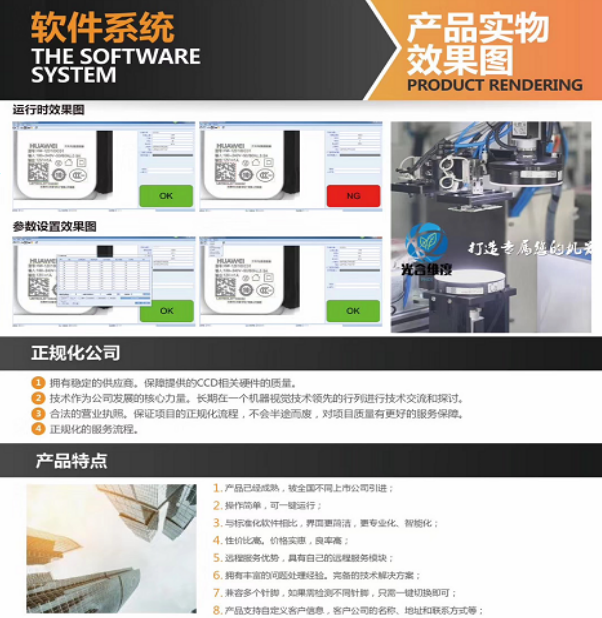
\includegraphics[width=\linewidth]{PrjMy_2.png}
			\end{minipage} 
			\hfill
			\begin{minipage}[th]{0.6\textwidth}
				\textbf{\underline{字符缺陷检测和识别系统}}
				\begin{enumerate}
					\item 对不同产品进行油墨缺陷检测.多印缺印,重影等检测。
					\item 字符识别
					\item 二维码识别
					\item 连接MES系统等
				\end{enumerate}
				\vfill
				\vspace{5em}
			\end{minipage}
		\bigskip
		\end{minipage}
		
		\vspace{2em}
		
		\begin{minipage}[thbp]{\textwidth}
		\begin{minipage}[thbp]{0.3\textwidth}
			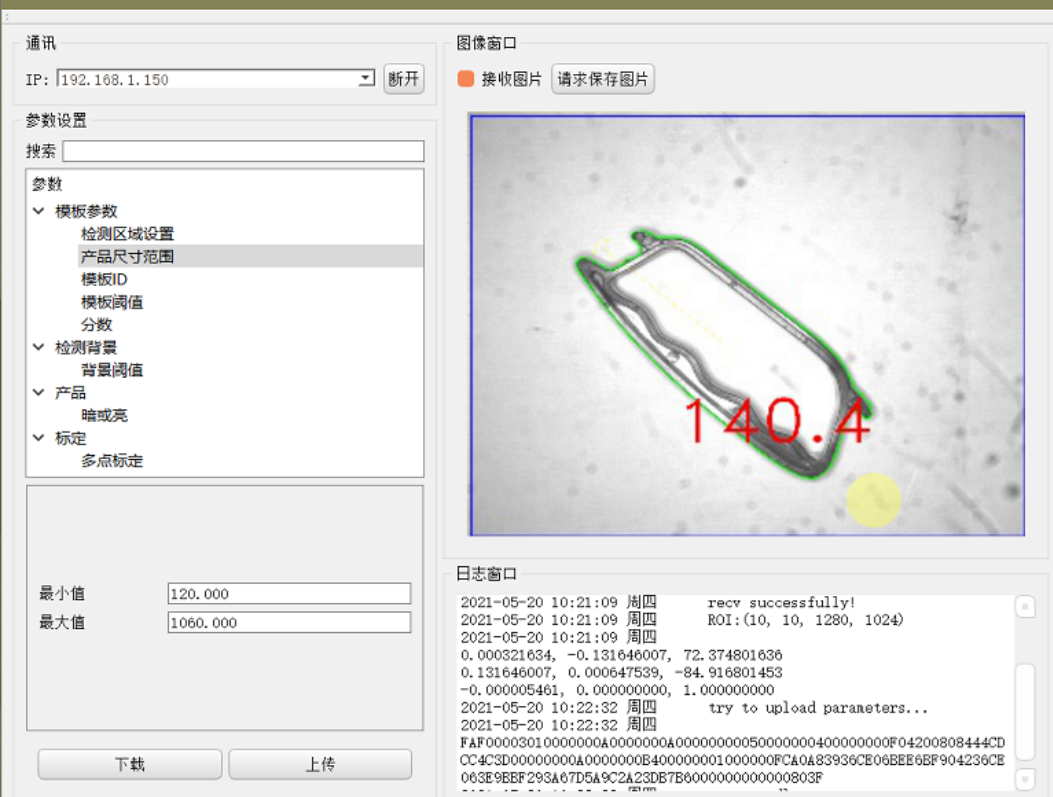
\includegraphics[width=\linewidth]{PrjMy_3.png}
		\end{minipage} 
		\hfill
		\begin{minipage}[thbp!]{0.6\textwidth}
			\textbf{\underline{流水线机器人传动带分拣系统}}
			\begin{enumerate}
				\item 360度形状匹配
				\item Python + OpenCV实现算法
				\item Qt实现上位机交互界面
				\item 解决显示模块效率问题
				\item 完成飞拍算法
			\end{enumerate}
		\end{minipage}
		\bigskip
		\end{minipage}
		
		\bigskip
	\end{minipage}
	
	\vspace{2em}
	\vfill{}
	
	\begin{minipage}[t]{\textwidth}
		\section*{技术分享文章(\hiddenlink{https://bbs.kanxue.com/homepage-940598.htm}{看雪论坛})}
		\begin{tabular}{>{\scriptsize\bfseries\linespread{1.6} \selectfont}l >{\footnotesize}p{0.55\textwidth}}
			
			二进制修复中文乱码的问题(161K+) & \href{https://zhuanlan.kanxue.com/article-16938.htm}{https://zhuanlan.kanxue.com/article-16938.htm} \\
			优化逆向编程环境(10K+ 优) & \href{https://bbs.kanxue.com/thread-276273.htm}{https://bbs.kanxue.com/thread-276273.htm} \\
			Qt,一个习惯引起的无效堆内存 & \href{https://bbs.kanxue.com/thread-275353.htm}{https://bbs.kanxue.com/thread-275353.htm} \\
			堆栈破坏-Windows下Qt调用MFC的DLL & \href{https://bbs.kanxue.com/thread-276097.htm}{https://bbs.kanxue.com/thread-276097.htm}
		\end{tabular}
		\bigskip
	\end{minipage}
	
	\vspace{3em}
	
	\vfill{} % Whitespace before final footer
	
	%----------------------------------------------------------------------------------------
	%	FINAL FOOTER
	%----------------------------------------------------------------------------------------
	\setlength{\parindent}{0pt}
	\begin{minipage}[t]{\linewidth}
		\begin{flushright}\fontfamily{\sfdefault}\selectfont \color{black!70}
			{\icon{\faMapMarker}{cvgreen}{} GuangDong/DongGuan \icon{\faPhone}{cvgreen}{} 13265599720 \icon{\faAt}{cvgreen}{} \protect\url{thinct_123@foxmail.com}
			}
		\end{flushright}
	\end{minipage}
	
\end{document}
